\documentclass[12pt]{article}

\usepackage{graphicx}			% Use this package to include images
\usepackage{amsmath}	
\usepackage{amsfonts}
\usepackage{polynom}
% A library of many standard math expressions
\graphicspath{ {./Images/} }
\usepackage[margin=1in]{geometry}% Sets 1in margins. 
\usepackage{fancyhdr}			% Creates headers and footers
\usepackage{enumerate}          %These two package give custom labels to a list
\usepackage[shortlabels]{enumitem}


% Creates the header and footer. You can adjust the look and feel of these here.
\pagestyle{fancy}
\fancyhead[l]{Aditya Gupta}
\fancyhead[c]{Math 134 Homework \#5}
\fancyhead[r]{\today}
\fancyfoot[c]{\thepage}
\renewcommand{\headrulewidth}{0.2pt} %Creates a horizontal line underneath the header
\setlength{\headheight}{15pt} %Sets enough space for the header



\begin{document} 
\begin{enumerate}[start=1,label={\bfseries. },leftmargin=1in]
\item [1. ]
A linear function $ f: \mathbb{R} \rightarrow \mathbb{R} $ is of the form:
\[
f(x) = ax + b
\]
For any \( x, y \in \mathbb{R} \):
\[
|f(x) - f(y)| = |(ax + b) - (ay + b)| = |ax - ay| = |a| |x - y|.
\]

Given $\epsilon > 0$, let \( \delta = \frac{\epsilon}{|a|} \) (given \( a \neq 0 \); otherwise, if \( a = 0 \), \( f(x) \) is a constant function, which is uniformly continuous).

Then, if \( |x - y| < \delta \), we have:
\[
|x-y| < \frac{\epsilon}{|a|}
\]
\[
|a||x-y| < \epsilon
\]

As per prior result
\[
|f(x) - f(y)| < \epsilon
\]

Thus, since $\delta$ is defined without depending on x, a linear function is uniform continuous.

\item [2.] 
\begin{enumerate}
    \item Prove that $x^2$ is uniform continuous on a bounded interval

    Consider the function \( f: \mathbb{R} \rightarrow \mathbb{R} \) defined by:
\[
f(x) = x^2
\]
For any \( x, y \in [a, b] \):
\[
|f(x) - f(y)| = |x^2 - y^2| = |(x - y)(x + y)| = |x - y| \cdot |x + y|.
\]

Since \( x, y \in [a, b] \), we have \( x + y \in [2a, 2b] \), so:
\[
|x + y| \leq 2|b|.
\]

Given \( \epsilon > 0 \), let \( \delta = \frac{\epsilon}{2|b|} \). Then, if \( |x - y| < \delta \), we have:
\[
|x - y| < \frac{\epsilon}{2|b|}
\]
\[
|x - y| \cdot 2|b| < \epsilon.
\]
\[
|x-y|\cdot|x+y| < \epsilon
\]

Thus, by the prior result, we have:
\[
|f(x) - f(y)| < \epsilon.
\]

Therefore, since \( \delta \) is defined independently of \( x \) and \( y \), \( f(x) = x^2 \) is uniformly continuous on the interval \( [a, b] \).

\item
Assume, for the sake of contradiction, that \( f(x) = x^2 \) is uniformly continuous on the real line.

This means that for every \( \epsilon > 0 \), there exists a \( \delta > 0 \) such that for all \( x, y \), if \( |x - y| < \delta \), then \( |f(x) - f(y)| < \epsilon \).

Let \( \epsilon = 1 \) and suppose there exists a corresponding \( \delta > 0 \). Consider any \( x \in \mathbb{R}\) and let \( y = x + \frac{\delta}{2} \). Then, we have:
\[
|x - y| = \left| x - \left( x + \frac{\delta}{2} \right) \right| = \frac{\delta}{2},
\]
which satisfies \( |x - y| < \delta \).

Now, evaluate \( |f(x) - f(y)| \):
\[
|f(x) - f(y)| = |x^2 - \left(x + \frac{\delta}{2}\right)^2|.
\]
Expanding \( (x + \frac{\delta}{2})^2 \), we get:
\[
\left(x + \frac{\delta}{2}\right)^2 = x^2 + x \delta + \frac{\delta^2}{4},
\]
so
\[
|f(x) - f(y)| = \left| x^2 - \left( x^2 + x \delta + \frac{\delta^2}{4} \right) \right| = |x \delta + \frac{\delta^2}{4}|.
\]

Since \( x \) can be chosen arbitrarily large, \( |x \delta + \frac{\delta^2}{4}| \) can be made arbitrarily large as well, which contradicts the requirement that \( |f(x) - f(y)| < \epsilon = 1 \).

Therefore, \( f(x) = x^2 \) is not uniformly continuous on an open interval.

\end{enumerate}
\item [12. ]
For an interval $[a,b]$, we take an arbitrary partition $P = [x_0, x_1, x_2,...,x_n]$ where:

\[
a = x_0 < x_1 < x_2 <...<x_{n-1}<x_n = b
\]

Since $f(x) = x + 3$ is a strictly increasing function,
\[
f(x_{i-1}) \leq f\left(\frac{x_{i-1} + x_i}{2}\right) \leq f(x_i)
\]
\[
x_{i-1} + 3 \leq \frac{x_{i-1}  +3 +x_i + 3 }{2} \leq x_i + 3
\]
Multiplying by $\Delta x$ on all sides. Since $\Delta x > 0$, no sign change is required
\[
\Delta x_i(x_{i-1} + 3) \leq (x_i - x_{i-1})\frac{x_{i-1}  +3 +x_i + 3 }{2} \leq(x_i + 3)\Delta x_i
\]
\[
\Delta x_i(x_{i-1} + 3) \leq \frac{(x_{i-1} +x_i) \cdot(x_i - x_{i-1})}{2} + 3\cdot(x_i - x_{i-1}) \leq (x_i + 3)\Delta x_i
\]
Summing from $i = 1\to n$,
\[
\sum_{i=1}^n\Delta x_i(x_{i-1} + 3) \leq \sum_{i=1}^n\frac{(x_{i-1} +x_i) \cdot(x_i - x_{i-1})}{2} + 3\cdot(x_i - x_{i-1}) \leq \sum_{i=1}^n(x_i + 3)\Delta x_i
\]
Since,
\[
L_f(P)=\sum_{i=1}^n\Delta x_i(x_{i-1} + 3)
\]
\[
U_f(P)=\sum_{i=1}^n\Delta x_i(x_{i} + 3)
\]

\[
L_f(P) \leq \frac{1}{2}\sum_{i=1}^n (x_i^2 - x_{i-1}^2) + 3\sum_{i=1}^n x_i - x_{i-1} \leq U_f(P)
\]

\[
L_f(P) \leq \frac{1}{2}( x_1^2 - x_0^2 + x_2 ^2 - x_1^2 + ... +x_n^2 - x_{n-1}^2) + 3(x_1 - x_0 + x_2 - x_1 + ... +x_n - x_{n-1})
\leq U_f(P)
\] 
The sums simplify to:
\[
L_f(P) \leq \frac{1}{2}(x_n^2 - x_0^2) + 3(x_n - x_0) \leq U_f(P)
\]

Since $x_0 = a$ and $x_n = n$,

\[
L_f(P) \leq \frac{1}{2}(b^2 - a^2) + 3(b-a)\leq U_f(P) 
\]

Thus:

\[
\int_{a}^b f(x)dx = \frac{1}{2}(b^2 - a^2) + 3(b-a)
\]

\item [32. ]

For an interval $[a,b]$, we take an arbitrary partition $P = [x_0, x_1, x_2,...,x_n]$ where:

\[
a = x_0 < x_1 < x_2 <...<x_{n-1}<x_n = b
\]

Since $f(x)$ is strictly decreasing on $[a,b]$,

\[
U_f(P) = \sum_{i=1}^n f(x_{i-1}) \Delta x 
\]
\[
L_f(P) = \sum_{i=1}^n f(x_{i})\Delta x 
\]
Expanding the sums:
\[
U_f(P) - L_f(P) = \Delta x((f(x_0) + f(x_1)+ ...+f(x_{n-1})) - (f(x_1) + f(x_2)+ ...+f(x_{n})))
\]
Subtracting common terms:
\[
U_f(P) - L_f(P) = \Delta x(f(x_0) - f(n))
\]
Thus proven:
\[
U_f(P) - L_f(P) = (f(a) - f(b))\Delta x
\]
\newpage

For the following 5 questions, the following identity will be repeated and will be referred to as the integral inequality for the purpose of this homework:
For an arbitrary partition P
\[
L_f(P) \leq \int_a^b f(x)dx \leq U_f(P)
\]
\[
L_g(P) \leq \int_a^b g(x) dx \leq U_g(P)
\]

Since $\int_a^b f(x)dx > \int_a^b g(x)dx$
The following integral inequality is necessarily true:
\[
L_g(P) \leq \int_a^b g(x)dx < \int_a^b f(x)dx \leq U_f(P)
\]

\item [25. ]
Following from the aforementioned integral inequality:
\[
L_g(P) < U_f(P)
\]

\item [26. ] Taking $f(x) = x$, $g(x) = 0.2$, $a = 0$, $b = 1$ and $P = \{0, 0.05, 1\}$.

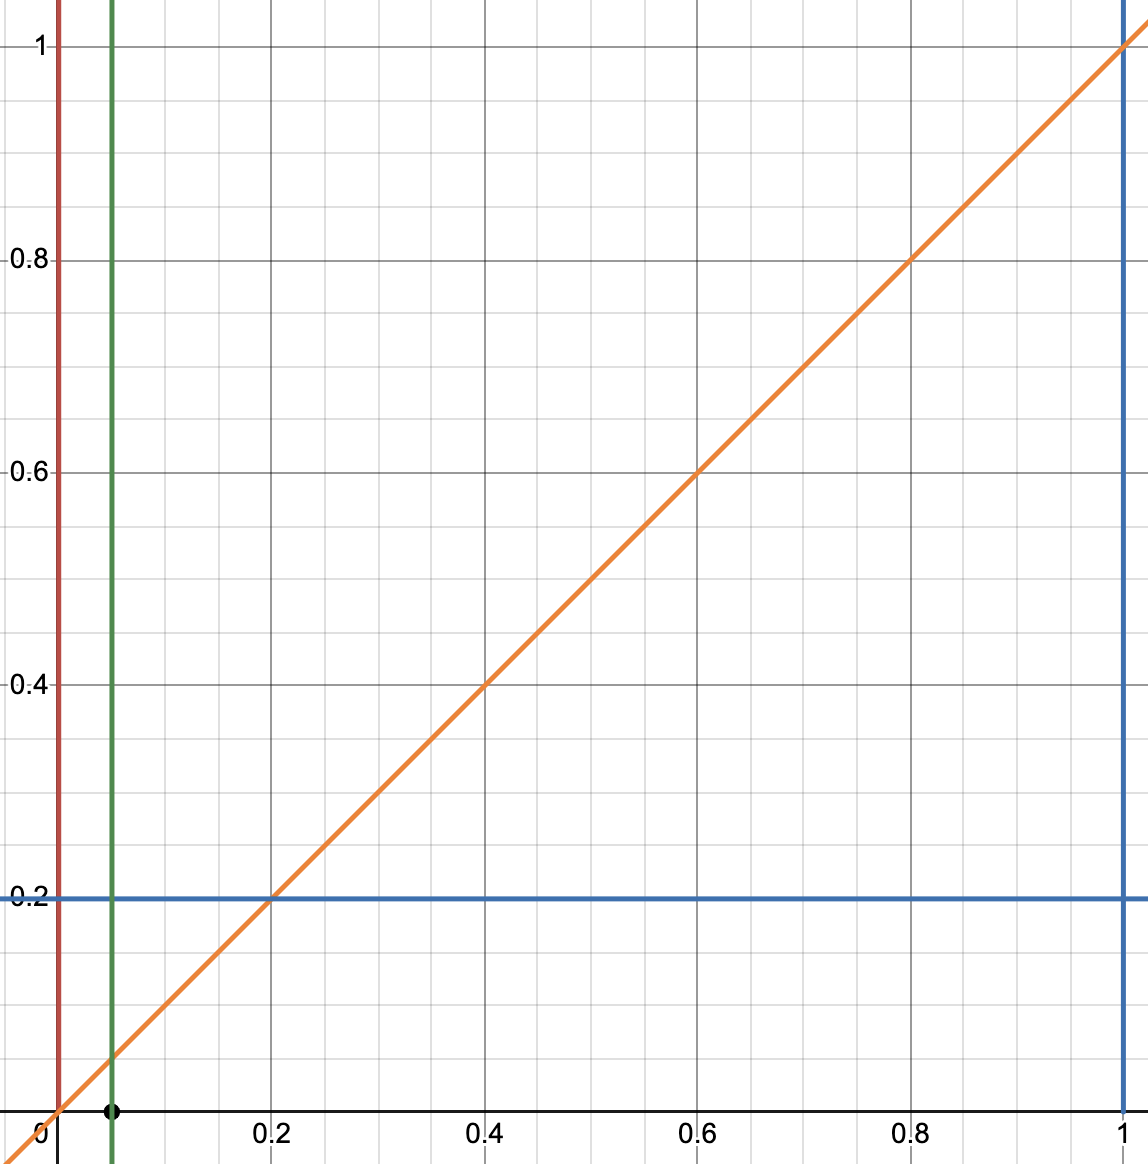
\includegraphics[width=0.75\linewidth]{Math 134//Images/26.png}

It is seen that the $L_f(P) < L_g(P)$ as $L_f(P) = (0.05\times0.95 ) = 0.0475$ whereas $L_g(P) = 0.2 \times 1 = 0.2$

\item [27. ]
Following from the aforementioned integral inequality:
\[
L_g(P) < \int_a^b f(x)dx
\]

\item [28. ] Taking $f(x) = 1$, $g(x) = x^{10}$, $a = 0$, $b = 1.02$ and $P = \{0, 0.05, 1\}$.

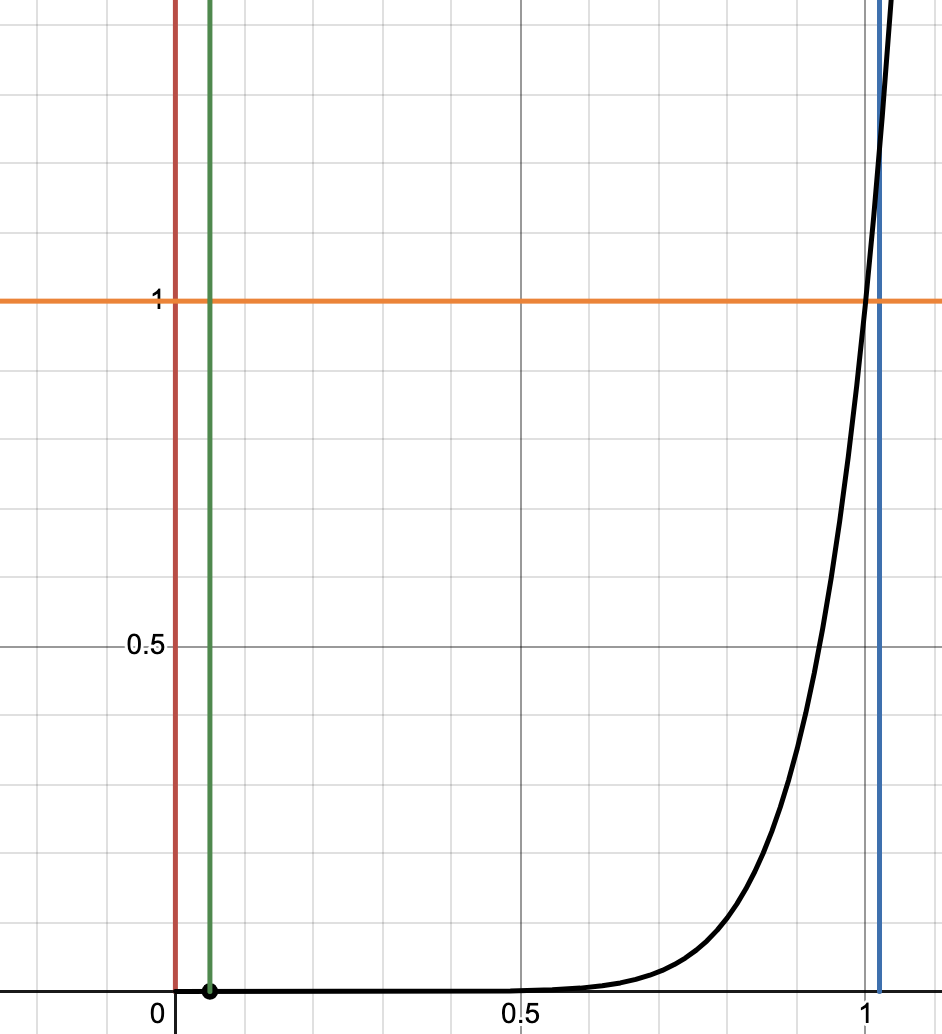
\includegraphics[width=0.5\linewidth]{Math 134//Images/28.png}

It is seen that the upper sum of $g(x)$ would be greater as it's suprenum on the $0.05, 1$ interval is greater than $f(x)$ and the other interval is minuscule.

\item [29. ]
Following from the aforementioned integral inequality:
\[
U_f(P) > \int_a^b g(x)dx
\]
\item [30. ]

We may refer to the example of Q.28. Since we proved an example of:
\[
U_g(P) > U_f(P) \text{ and because } U_f(P) \geq \int_a^bf(x) dx
\]
We can say:
\[
U_g(P) > \int_a^bf(x) dx
\]

\end{enumerate}
\end{document}
